% !TeX root = ../main.tex
\chapter{提案手法}
\label{chap:method}

\section{システムの構成}
\label{sec:system}
% 図の参照は Fig.~\ref{fig:...}．~ は改行させない空白
これは記入例のためのダミーの文である．
システムの概要をFig.~\ref{fig:overview}に示す．

% 図：ファイルは fig/ に置き，fig/ から書く．配置の指定は [t]
\begin{figure}[t]
  \centering
  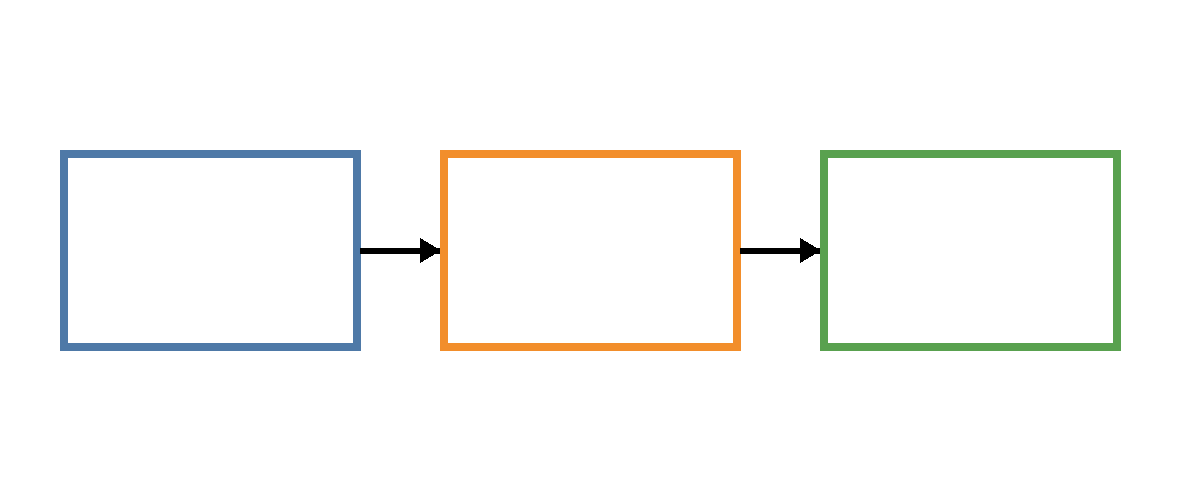
\includegraphics[width=0.8\linewidth]{fig/overview.png}
  \caption{システムの概要}
  \label{fig:overview}
\end{figure}

\section{距離の計算}
\label{sec:distance}
% 文中の数式は $ で囲む
2点$p = (x_1, y_1)$，$q = (x_2, y_2)$の距離$d$を，式\eqref{eq:distance}で求める．

% 番号付きの数式．参照は \eqref{eq:...}
\begin{equation}
  d = \sqrt{(x_1 - x_2)^2 + (y_1 - y_2)^2}
  \label{eq:distance}
\end{equation}

% 複数行の数式は align で，= の前に & を置いてそろえる
\begin{align}
  v &= \frac{d}{t} \label{eq:velocity} \\
  a &= \frac{\Delta v}{\Delta t} \label{eq:acceleration}
\end{align}

\section{前処理}
\label{sec:preprocess}
これは記入例のためのダミーの文である．
処理の前後の画像をFig.~\ref{fig:beforeafter}に，処理後の画像をFig.~\ref{fig:after}に示す．

% 図の横並び：subfigure 環境を並べる
\begin{figure}[t]
  \centering
  \begin{subfigure}{0.45\linewidth}
    \centering
    
\includegraphics[width=\linewidth]{fig/before.png}
    \caption{処理前}
    \label{fig:before}
  \end{subfigure}
  \hfill
  \begin{subfigure}{0.45\linewidth}
    \centering
    
\includegraphics[width=\linewidth]{fig/after.png}
    \caption{処理後}
    \label{fig:after}
  \end{subfigure}
  \caption{処理の前後の画像}
  \label{fig:beforeafter}
\end{figure}
